\chapter{跨软件生态的兼容性问题实证研究}
在Ubuntu系统中,用户管理Python第三方包的最常见方式是利用apt和pip等包管理工具,二者会在系统内维护自身软件生态的第三方包仓库。在实际软件开发中,两个软件仓库的Python第三方包之间会发生的兼容性问题,在本文中将其称为跨软件生态的兼容性问题,简称CC问题。CC问题是包管理工具在包安装期间无法被检测到的,而CC问题导致软件发生错误后,报错信息和传统包兼容性问题十分相似,这导致用户难以解决CC问题。那么,CC问题是什么表现形态以及是如何发生的呢?为了探讨这一问题,本章针对CC问题进行了实证研究。具体而言,本章从CC问题的发生原因,CC问题的特征,CC问题对系统的影响三方面展开了广泛的分析研究。最终,本章分析了CC问题发生的根本原因,并总结了CC问的三种触发模式和四种故障症状。在此基础上,本章通过测试的方法,研究了CC问题对于Ubuntu20.04系统的影响,并构建了一个包括1692个CC问题的数据库。这些发现对于后续设计和评估检测工具起到了强有力的支撑作用。

\section{研究动机和问题}
本节首先介绍第三方包依赖管理的一些背景知识,引出一个CC问题的问题实例,之后介绍相关研究工作在解决CC问题上的不足,最终提出分析CC问题的研究问题。
\subsection{研究动机}
软件包管理工具被广泛用于管理软件依赖性,并自动化软件包安装过程。许多编程语言社区提供了各自的管理工具,例如,pip 负责管理近 50 万个 Python 软件包 \upcite{pip},而 npm 则管理超过 300 万个 JavaScript 软件包\upcite{npm}。此外,操作系统社区也提供了诸如 apt 和 dnf 等管理工具,这些工具管理的是操作系统发行版的软件包,而非特定编程语言的软件包。例如,在 Debian/Ubuntu 等发行版中,apt 能够管理包括但不限于 C/C++/Python/JavaScript 的 deb 软件包 \upcite{apt}。同样,在 RHEL/Fedora 等发行版中,dnf 可以管理不同编程语言的 rpm 软件包 \upcite{Fedora}。

软件包管理工具本身通常都经过精心设计,以处理其自身仓库中软件包的依赖关系。为实现这一点,仓库通常要求其软件包明确指定依赖的软件包及其相应的版本范围。然而,从终端用户的角度来看,他们经常需要跨不同仓库的多个软件包。例如,Ubuntu 用户可能会交替使用 apt 和 pip。在这些情况下,可能会出现兼容性问题。
\begin{figure}[htbp] % use float package if you want it here
	\centering
	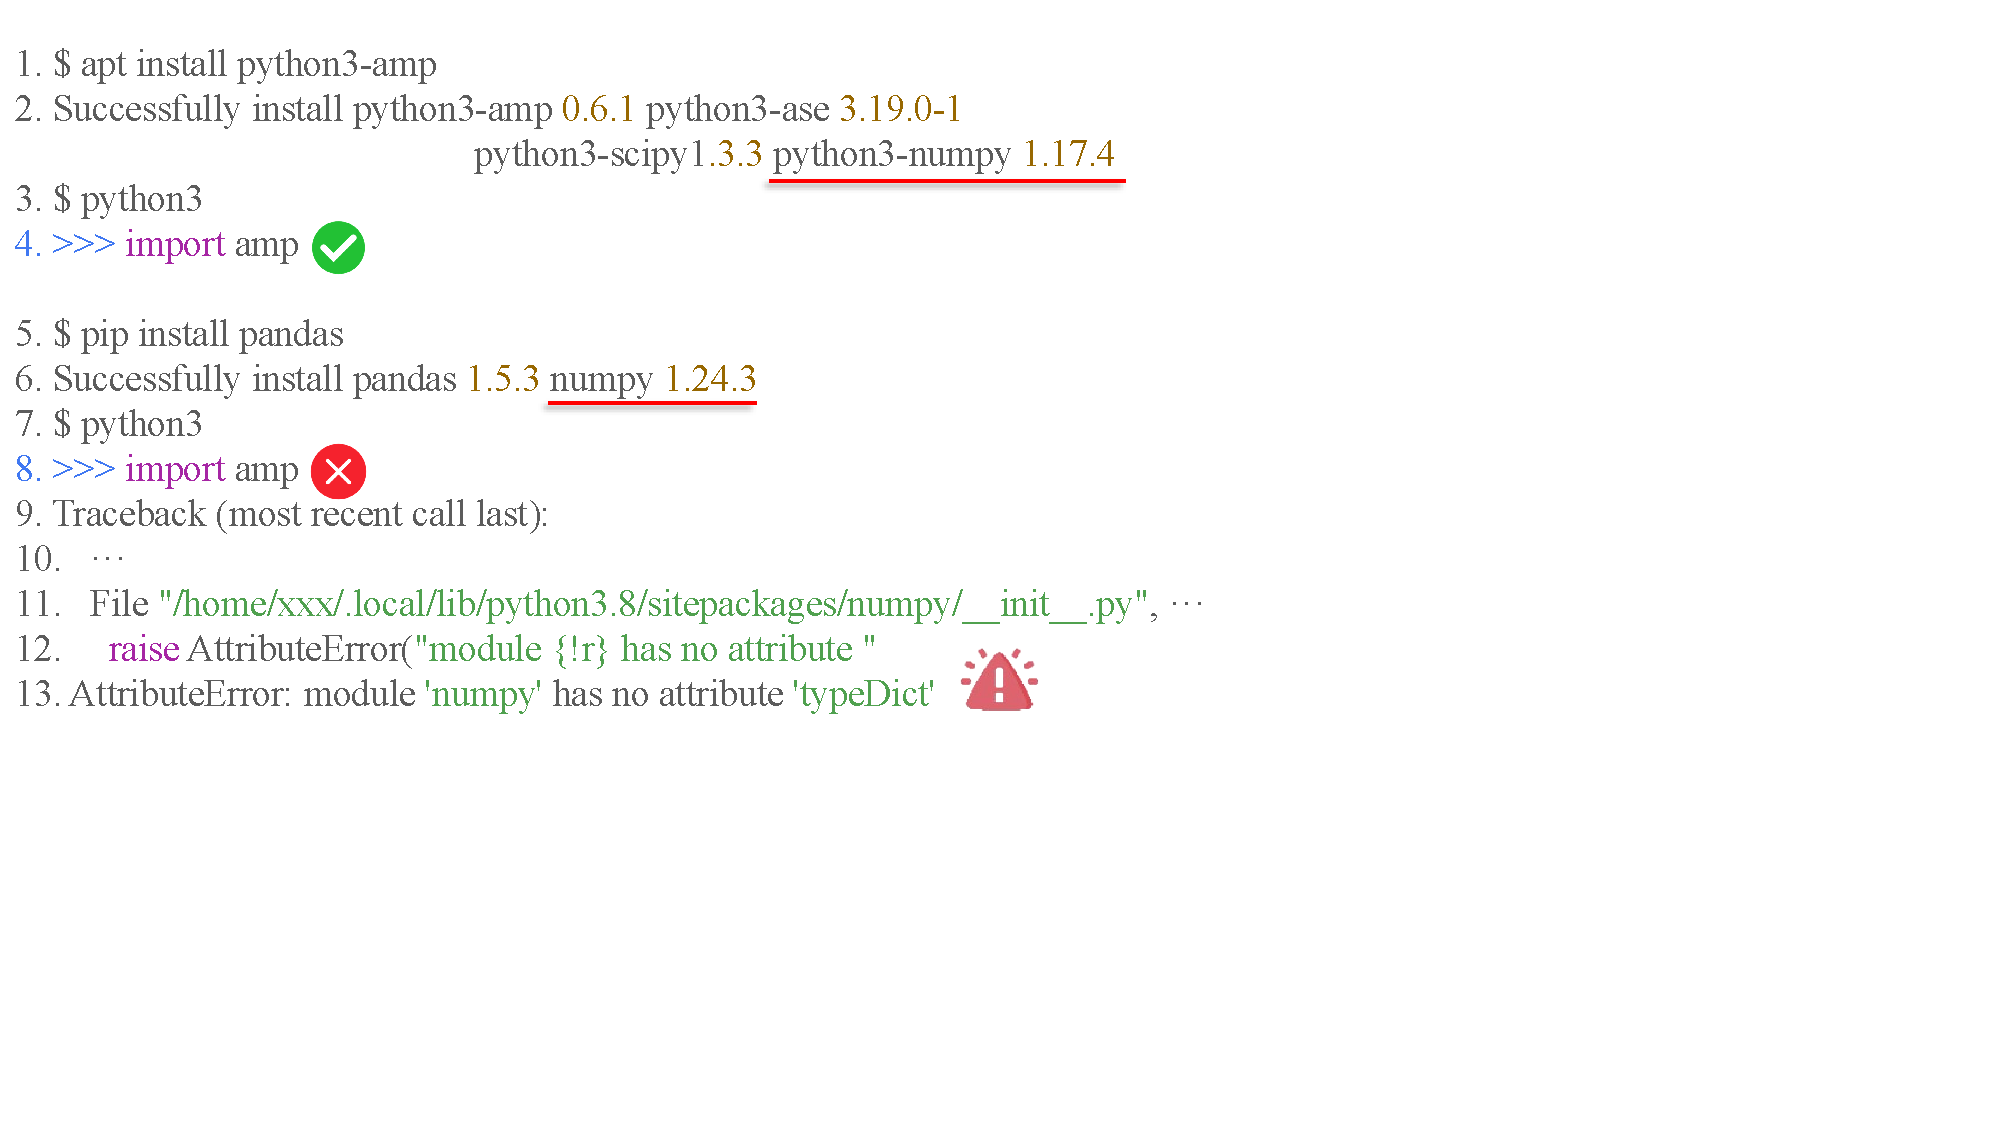
\includegraphics[width=5in]{introduction1}
	\caption{由于在 Ubuntu 中混合使用 apt 和 pip 安装而导致的第三方包不兼容问题}
	\label{fig:example}
\end{figure}
图\ref{fig:example}展示了一个真实案例,其中包含了一系列使用不同管理工具安装 Python 软件包的命令。第 1 行使用 apt 安装了 “amp 0.6.1”(一个原子级机器学习软件包)及其依赖项 “ase 3.19.0-1”、 “scipy 1.3.3” 和 “numpy 1.17.4”。此时,“amp” 可以正常导入(第 3-4 行)。随后,第 5 行使用 pip 安装了 “pandas 1.5.3” 及其依赖项 “numpy 1.24.3”。安装后,“amp” 无法再被正常导入(第 7-8 行)。根据回溯信息显示,“amp” 与位于 “/home/xxx/.local/lib/python3.8/site-packages/”的 “numpy” 不兼容,即 pip 的安装路径。这意味着,当导入通过 apt 安装的 “amp 0.6.1” 时,Python 解释器会导入通过 pip 安装的 “numpy 1.24.3”,而不是 apt 安装的 “numpy 1.17.4”,从而导致兼容性问题。本文中将此类问题称为跨软件生态的兼容性问题,简称CC问题。

针对兼容性问题的研究由来已久,大致可以分为两大类。首先,许多研究致力于检测依赖冲突(即一个软件包依赖于另一个软件包的两个冲突版本)\upcite{wang2022smartpip,wang2020watchman,lieasypip,wang2023automatically,cao2024diagnosis,wang2018dependency,wang2019could,wang2021will,patra2018conflictjs}以及依赖解析(即是否存在与所有已安装软件包兼容的软件包版本)\upcite{abate2020dependency,trezentos2010apt,abate2012dependency}。前者通常应用于特定编程语言社区(例如 Python、JAVA、JavaScript),而后者则主要针对操作系统发行版。所有这些研究都难以处理CC问题。其次,有些研究使用测试或程序分析技术来检测软件包兼容性(即给定版本的两个软件包是否彼此兼容)\upcite{mezzetti2018type,moller2019model,ponomarenko2012backward,zhang2020python,chen2020taming,jia2021depowl}。这些研究能够判断依赖软件包的指定版本范围(通常在软件包规范文件中)是否包含不兼容的版本。然而,即使所有仓库中的版本范围均正确,也仍然会发生CC问题。
\subsection{研究问题设置}
为了深入分析CC问题,以便后续设计自动化解决工具,本章从以下三个研究问题对CC问题展开实证研究:
\begin{itemize}
	\item \textbf{RQ1:}跨软件生态的兼容性问题发生的根本原因是什么?(根本原因)
	\item \textbf{RQ2:}跨软件生态的兼容性问题相比于其他兼容性问题的特征是什么?(问题特征)
	\item \textbf{RQ3:}跨软件生态的兼容性问题对于系统的影响有多大?(问题影响)
\end{itemize}

\section{RQ1:根本原因}
所有CC问题都涉及使用第三方包的两个重要阶段:安装和导入第三方包。为了分析CC问题的根本原因,本节首先分析Python第三方包的安装和导入策略,然后分析图\ref{fig:example}背后的系统各个第三方包仓库的状态和包导入状态,最终总结CC问题的根本原因。

\subsection{Python第三方包的安装策略}
在像 Ubuntu 这样的操作系统发行版中,用户可以使用 apt 或 pip 来安装 Python 软件包。
这些工具最重要的步骤是找到满足指定版本约束的所需软件包及其依赖项的合适版本,这一过程也被称为依赖解析 \upcite{wang2022smartpip}。
一方面,apt 在其自身目录中进行依赖解析,如果目录中未找到所需的软件包版本,则会安装一些特定的版本。
这些版本是预先定义的,与操作系统发行版的版本相对应 \upcite{abate2020dependency}。
另一方面,pip 通过扫描所有系统级 Python 目录来解析依赖 \upcite{pip_doc},并且:a) 如果在任何目录中未找到所需的软件包,pip 将默认安装最新版本;b) 如果找到软件包且其版本满足约束条件,pip 将不会进行任何操作;c) 如果找到的软件包版本不合适,pip 将替换为合适的版本(当软件包位于 pip 目录中时),或者只安装合适版本而不移除旧版本(当软件包位于其他目录中时)。

总而言之,apt 在安装软件包时不会考虑 pip 是否已经安装了该软件包。
因此,当交替使用 apt 和 pip 时,不同目录中存在不同版本的软件包是很常见的现象。

\subsection{Python第三方包的导入策略}
在导入软件包时,Python 解释器会依次在多个软件包目录中进行搜索,以找到所需的软件包\upcite{pip_doc}。
用户可以通过“sys.path”查看解释器使用的所有目录。
\begin{figure}[htbp] % use float package if you want it here
	\centering
	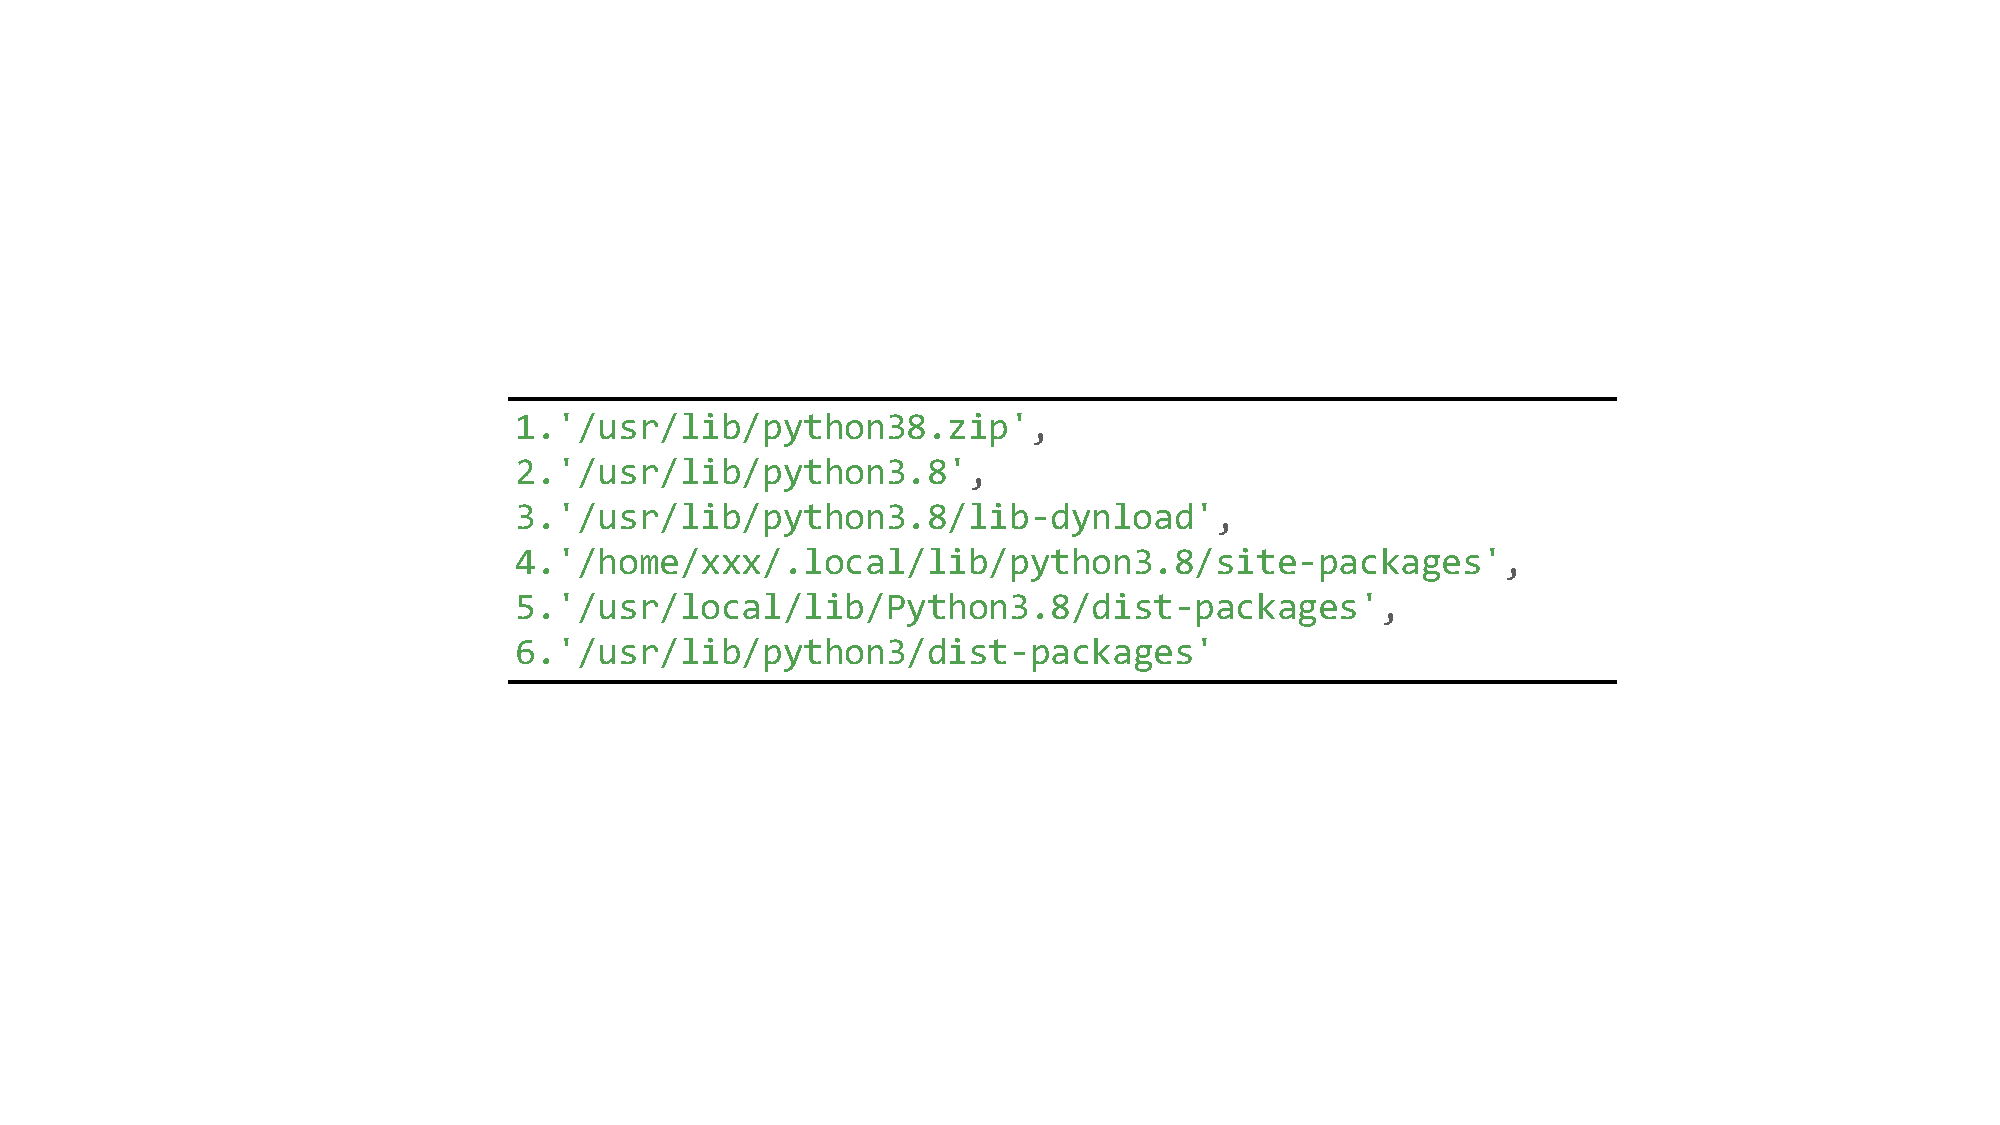
\includegraphics[width=5in]{import order}
	\caption{Ubuntu 系统中 Python 解释器的默认搜索顺序}
	\label{fig:order}
\end{figure}
图\ref{fig:order}展示了 Ubuntu 系统中 Python 解释器的默认搜索顺序。前两个是 Python 标准库目录(第 1-2 行),分别存储了压缩和未压缩的标准库。第三个目录用于存放动态加载的已编译扩展模块(第 3 行)。其余目录为第三方软件包目录,包括 pip 用户级目录(第 4 行)、pip 系统级目录(第 5 行)以及 apt 系统级目录(第 6 行)。用户级和系统级目录分别存储了普通用户和 root 用户安装的软件包。Python 解释器按照目录顺序根据软件包名称进行搜索,并采用查找即导入的策略,即一旦找到软件包便不再继续搜索后续目录。如果未找到该软件包,解释器将会报出“ImportError” 错误。

总而言之,Python 解释器默认优先从 pip 目录而非 apt 目录中导入软件包,而不会考虑版本问题。因此,当系统中存在多个版本时,可能会导入错误的版本。

\subsection{根本原因分析}
每个仓库都有其专属的管理工具,具备独特的软件包安装策略和目录结构。该工具通常都经过精心设计,用于处理仓库内部的依赖关系,而不会考虑跨仓库的依赖关系。
与此同时,Python 解释器会从两个仓库中导入软件包。
因此即使 apt、pip 和 Python 解释器均按预期工作,用户仍可能遇到图\ref{fig:example}中所示的兼容性问题。
\begin{figure}[htbp]
	\centering
	\subfloat[安装 pandas 之前的依赖导入情况]{
		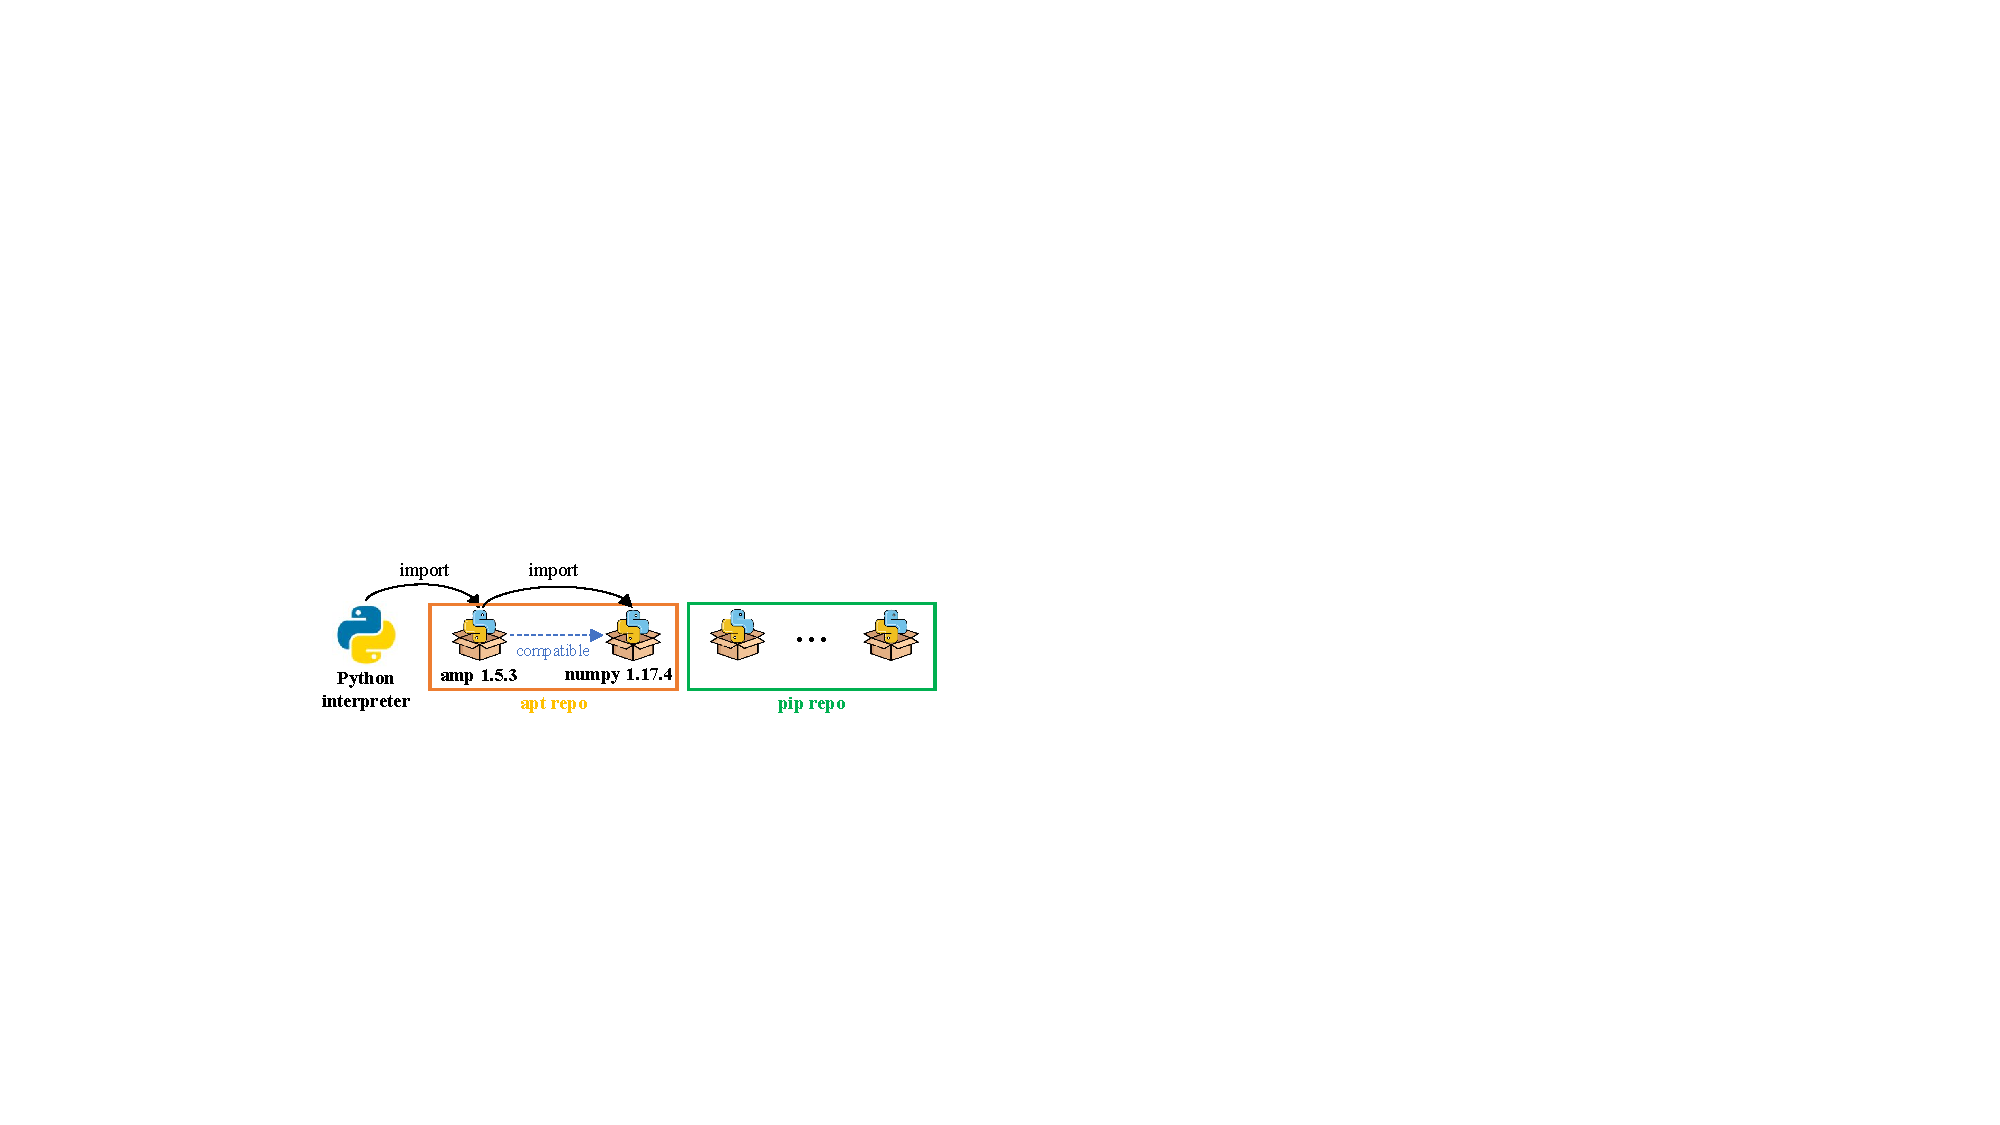
\includegraphics[width=.85\textwidth]{fig2-a.pdf}
		\label{fig:2-1}
	}\hspace{4em}
	\subfloat[安装 pandas 之后的依赖导入情况]{
		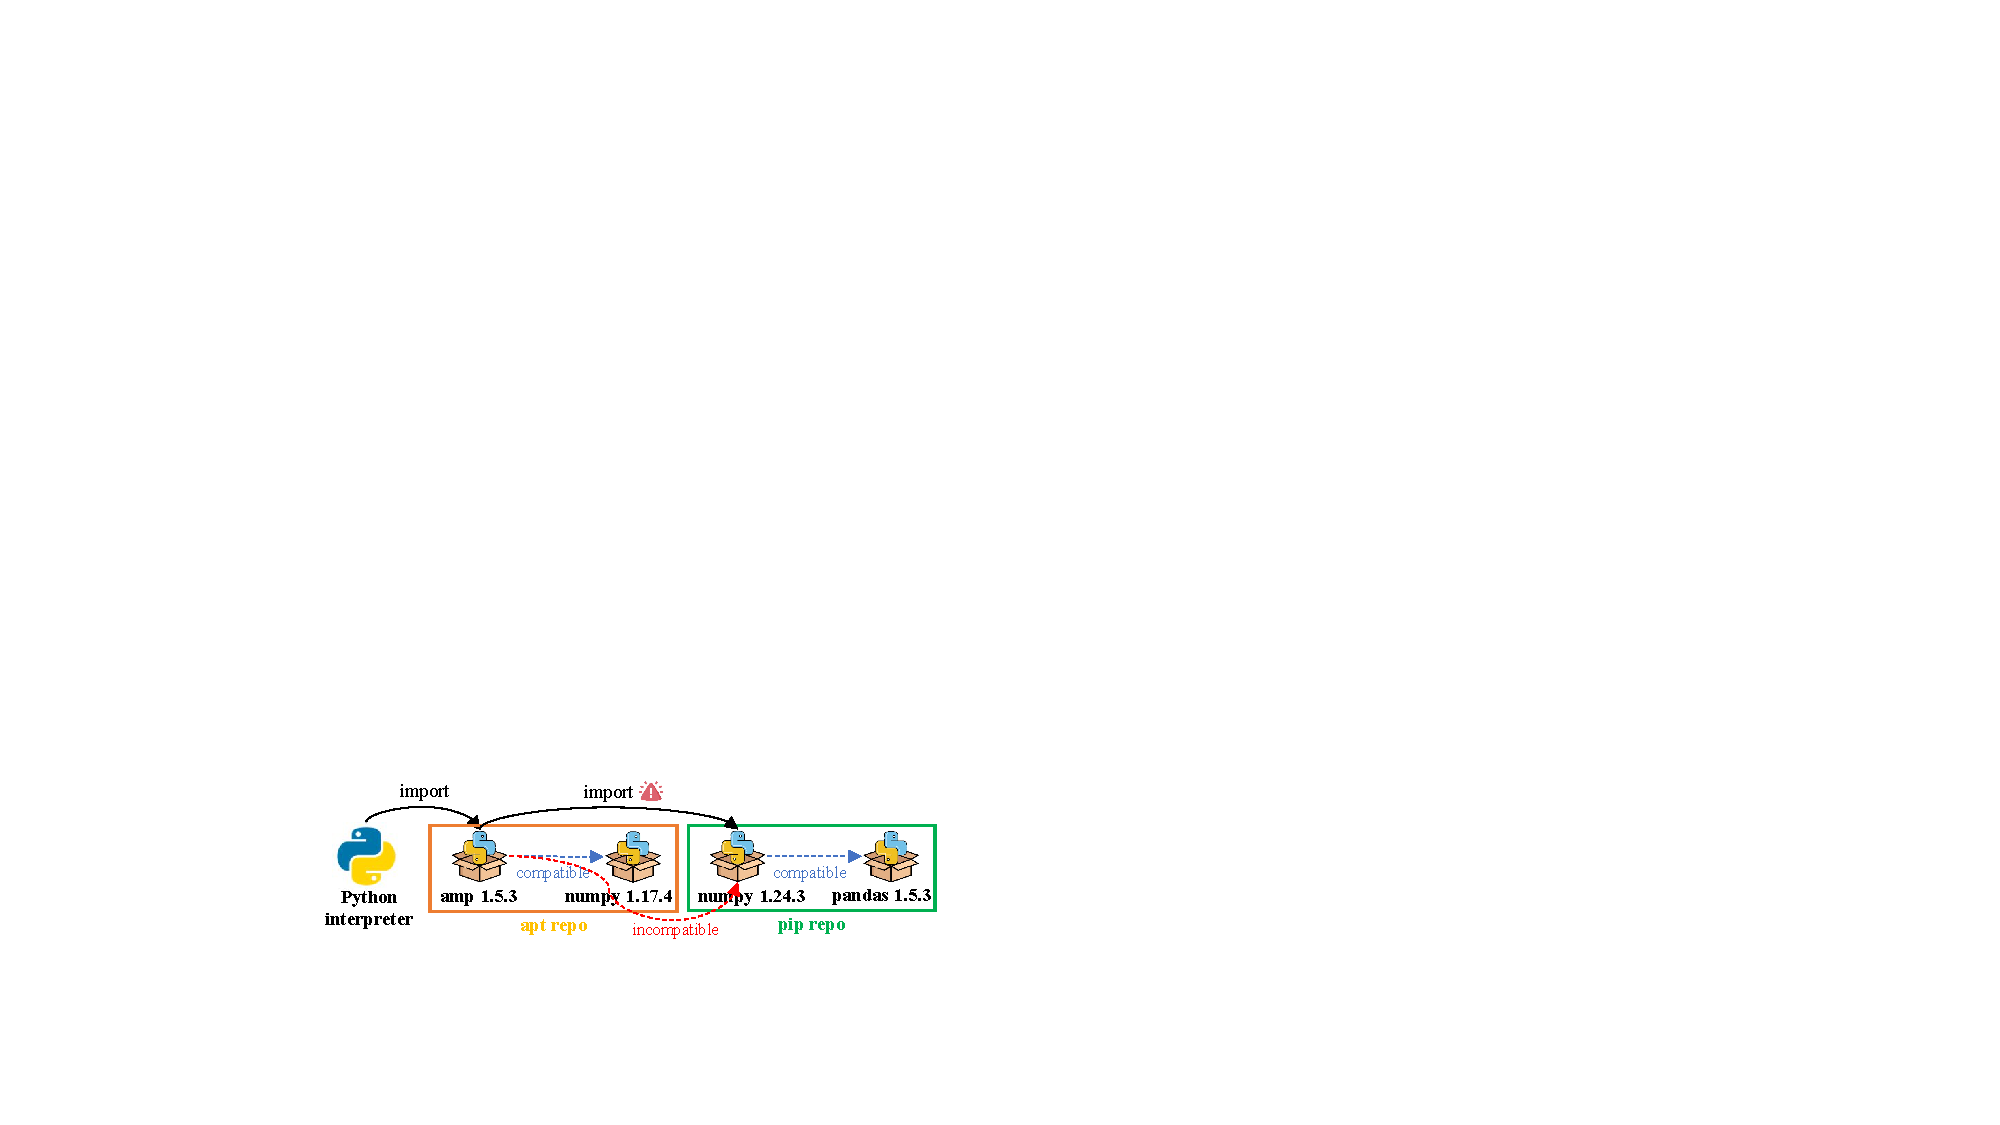
\includegraphics[width=.85\textwidth]{fig2-b.pdf}
		\label{fig:2-2}
	}
	\caption{图\ref{fig:example}中的CC问题的根本原因}
	\label{fig:2}
	% \vspace{-2mm}
\end{figure}
图\ref{fig:2}展示了该例子的根本原因。当使用 apt 安装 “amp” 时,Python 解释器将从 apt 仓库中导入 “numpy 1.17.4” 作为 “amp” 的依赖项,如图\ref{fig:2-1}所示。使用 pip 安装 “pandas” 后,导入的依赖关系如图\ref{fig:2-2}所示。此时,由于 Python 解释器的导入规则,来自 pip 仓库的 “numpy 1.24.3” 被视为 “amp” 的依赖项。然而,“numpy 1.24.3” 已经移除了 \textit{numpy.typeDict} 属性,导致了 CC 问题的发生。

\begin{tcolorbox}[boxrule=1pt,boxsep=1pt,left=2pt,right=2pt,top=2pt,bottom=2pt]
	\small
	\textcolor{red}{\faIcon{user-edit}} \noindent\textbf{RQ1结论:} 
	正常使用 apt、pip 和 Python 解释器可能会引发如图\ref{fig:example}所示的 CC 问题。因此,用户可能会频繁遇到这些问题。然而,很难单独归咎于 apt、pip 或解释器中的任何一方,因为它们都在按预期工作。CC 问题的根本原因在于 apt 和 pip 未考虑系统中的全局依赖关系,而 Python 解释器在执行过程中导入的依赖项与第三方包管理工具解析的依赖项存在差异。
\end{tcolorbox} 

\section{RQ2:问题特征}\label{3.3}
基于上述对CC问题根本原因的研究,本节进一步总结CC问题相对于其他兼容性问题的问题特征。本节从触发模式和故障表现两方面分析CC问题特征。在触发模式方面,本节总结了导致CC 问题的三种安装命令触发模式,如表\ref{tab:pattern}所示。
\begin{table}[htbp]
	\centering
	\small
	\begin{threeparttable}
		\caption{三种导致CC问题的触发模式}
		\label{tab:pattern}
		\begin{tabularx}{0.75\textwidth}{|c|>{\hsize=0.8\hsize}X|>{\hsize=1.2\hsize}X|}
			\hline
			\textbf{序号} & \textbf{命令模式} & \textbf{描述} \\ \hline
			1 & \begin{minipage}[t]{\linewidth}
				\textit{pip install B} \\
				\textit{apt install A}
			\end{minipage} & \textit{B}的默认安装版本和\textit{A}的默认安装版本不兼容。 \\ \hline
			2 & \begin{minipage}[t]{\linewidth}
				\textit{apt install A} \\
				\textit{pip install B==version}
			\end{minipage} & \textit{B}的\textit{version}版本和\textit{A}的默认安装版本不兼容。 \\ \hline
			3 & \begin{minipage}[t]{\linewidth}
				\textit{apt install A} \\
				\textit{pip install C}
			\end{minipage} & \textit{B}和\textit{A}一起安装的\textit{B}的版本不满足\textit{C}的依赖版本约束, 因此\textit{pip}安装一个新的\textit{B}并且这个版本\textit{B}和\textit{A}不兼容。 \\ \hline
		\end{tabularx}
		\begin{tablenotes}[flushleft]
			\item 假设有Python第三方包 \textit{A}、\textit{B}和\textit{C}, 其中 \textit{A} 和\textit{C} 依赖于 \textit{B}。
		\end{tablenotes}
	\end{threeparttable}
\end{table}
这三种模式均为用户在安装Python第三方包时经常使用的安装命令序列,通过这种安装方式,对在系统的不同仓库中安装同一个库包的不同版本,进而由于Python解释器的导入规则,可能引发CC问题。

基于上述分析,在故障表现方面,本节进一步总结了CC 问题的以下四种故障表现:
\begin{itemize}
	\item[a)] 应用包始终位于 apt 仓库中;
	\item[b)] 库包始终同时存在于 apt 和 pip 仓库中;
	\item[c)] 应用包与 apt 仓库中的库包兼容;
	\item[d)] Apt 仓库中的库包与 pip 仓库中的同名第三方包不兼容。
\end{itemize}


\begin{tcolorbox}[boxrule=1pt,boxsep=1pt,left=2pt,right=2pt,top=2pt,bottom=2pt]
	\small
	\textcolor{red}{\faIcon{user-edit}} \noindent\textbf{RQ2结论:} 
	CC问题相对于其他包兼容性问题,触发模式和故障表现不同。本节总结了三种触发模式和四种故障表现,这些模式和故障表现可以为\tool{}的设计和评估提供指导:a)本研究这些触发模式在构建真实场景的 CC 问题数据集;b)本研究使用这些故障表现来构建\tool{}设计过程中的依赖和兼容性表格。其中“apt 目录中始终存在兼容软件包”这一事实可以帮助\tool{}解决 CC 问题。
\end{tcolorbox} 

\section{RQ3:问题影响}\label{3.4}
为了研究CC问题对系统的影响严重程度,本节将探讨CC问题对于Ubuntu20.04系统的影响。具体而言,本节首先从Ubuntu20.04系统的apt软件仓库中的全部Python包出发,结合依赖关系和PyPI软件仓库中的Python包,构建可能触发CC问题的应用包与库包的组合和对应的安装命令。然后逐一测试执行安装命令,通过原本可以正常导入的Python第三方包是否在执行命令后导入失败来判断CC问题,之后收集整理发生的CC问题以构建一个CC问题数据集。在实际用户环境中,这些失败可能会导致正常运行的系统软件崩溃。

\subsection{组合构建}
首先,我们从 apt 仓库中收集了应用包。Ubuntu 20.04 维护了共计 3319 个 Python 第三方包,这些包都可以作为应用包。接着我们分析了每个应用包是否也存在于 pip 仓库中。具体而言,我们从 PyPI 中检索了每个应用包的可安装版本。如果存在可安装版本,我们将其视为库包,通过这种方式我们共获得了2419个库包。

在本节中,我们将用\textit{(A,B)}来表示每个应用包和库包的组合,其中\textit{A}代表来自apt仓库的应用包,\textit{B}代表来自pip仓库的库包。我们基于以下条件来构建组合:
\begin{itemize}
	\item \textbf{条件1:}第三方包\textit{A} 应为一个应用包,并且依赖于至少一个其他应用包;
	\item \textbf{条件2:}第三方包 \textit{B} 应同时存在于 apt 和 pip 仓库中,并且是 \textit{A} 的直接依赖或传递依赖。
\end{itemize}
基于apt软件源内部的依赖关系和条件1,我们识别了1917个依赖于至少一个其他应用包的应用包,这些包是有可能收到CC问题影响的应用包,占全部应用包的58\%。基于上述得到的库包和条件2,我们共构建了23866个可能发生CC问题的应用包与库包的组合。

\subsection{CC问题测试}
为测试每个软件包配对是否会遇到 CC 问题,我们使用了第\ref{3.3}节中触发模式1设计了图\ref{fig:command}所示的测试命令。
\begin{figure}[htbp] % use float package if you want it here
	\centering
	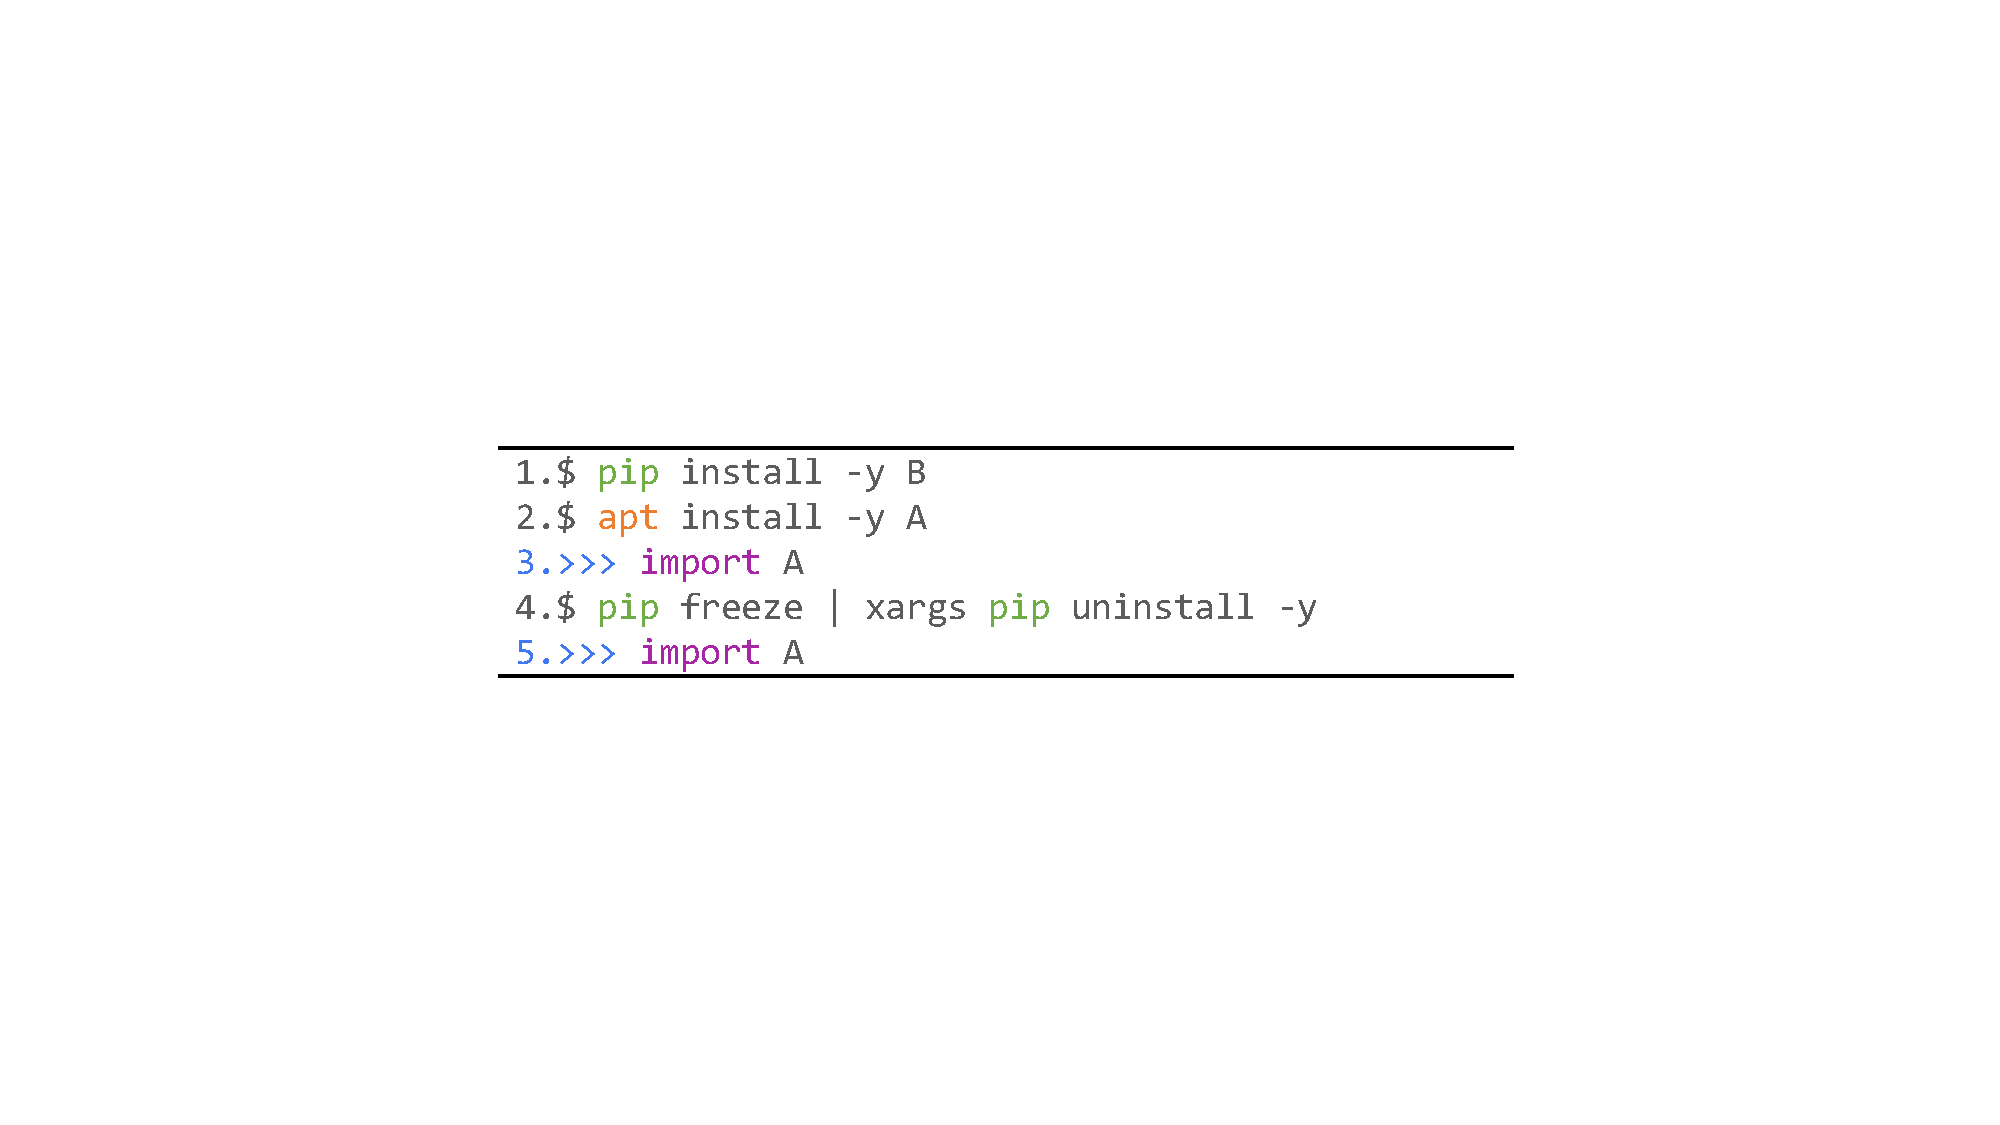
\includegraphics[width=5in]{commands}
	\caption{用于测试CC问题的命令序列}
	\label{fig:command}
\end{figure}
我们使用 Docker \upcite{docker} 来执行这些命令,以确保一个干净的系统环境。首先,我们分别使用 pip 和 apt 安装 \textit{B} 和 \textit{A}(第 1-2 行)。其次,我们在 Python 解释器中导入 \textit{A}(第 3 行)。如果导入失败导致崩溃,我们将卸载 pip 目录中的所有软件包,并再次导入 \textit{A}(第 4-5 行)。如果 \textit{A} 能够正常导入,这说明 \textit{B} 导致 \textit{A} 无法导入,并且 \textit{(A, B)} 存在 CC 问题。此外,我们还分析了回溯信息,以提取导致崩溃的破坏性 API。

总体而言,我们测试了所有 23,866 对组合,识别出了 1,692 对(7\%)存在 CC 问题的组合。
\begin{table}[htbp]
	\centering
	\begin{threeparttable}
		\caption{CC问题数据集}
		%\small
		\label{tab:CC}
		\begin{tabularx}{0.95\textwidth}{Xccccc}
			\toprule
			\textbf{组}&\textbf{Python第三方包}&\textbf{平均依赖}&\textbf{组合}&\textbf{崩溃}&\textbf{破坏性API} \\
			\midrule
			G1 [1,5]&1,048&2.24&2,234&89&82\\
			G2 [6,10]&282&7.80&2,189&261&255\\
			G3 [11,20]&218&14.60&2,322&91&89\\
			G4 [21,49]&211&31.96&6,751&677&674\\
			G5 [50,$+\infty$]&158&89.84&10,370&574&574\\
			\midrule
			\textbf{总数/平均} &1,917&14.96&23,866&1,692&1,674\\
			\bottomrule
		\end{tabularx}
	\end{threeparttable}
\end{table}
CC 问题数据集的统计结果如表\ref{tab:CC}所示,依赖关系较多的应用包相对更容易出现 CC 问题。我们成功从回溯信息中提取了 1,674 个(98.9\%)破坏性 API。在 18 个(1.1\%)未成功的案例中,有 11 个是由于软件包与 Python 解释器不兼容引起的,而 7 个则因回溯信息中缺乏明确的破坏性 API 信息。

\begin{tcolorbox}[boxrule=1pt,boxsep=1pt,left=2pt,right=2pt,top=2pt,bottom=2pt]
	\small
	\textcolor{red}{\faIcon{user-edit}} \noindent\textbf{RQ3结论:} 
	在Ubuntu20.04系统的系统软件源中,有1917个Python第三方包可能因CC问题而发生崩溃等严重问题。在构建的23866个组合中,尽管只有1692个通过测试发现了CC问题,但这不代表CC问题的发生概率小,这是因为我们的测试判断标准是执行导入命令失败,这不会运行应用包全部的代码分支,会导致许多CC问题没有被触发,后续的评估部分会详细阐述这一点。在实际用户环境中,这些CC问题可能会导致正常运行的系统软件崩溃,并且CC问题发生时的错误信息和传统包兼容性问题类似,导致用户难以排查并解决问题,最终对系统产生巨大影响。
\end{tcolorbox} 

\section{本章小结}
本章对CC问题进行了全面探讨,分析了在Ubuntu系统中使用apt和pip管理Python第三方包时出现的第三方包兼容性问题。通过实证研究,本章揭示了CC问题的成因、特征,并构建了包含1692个案例的CC问题数据库。研究发现,CC问题发生的根本原因在于 apt 和 pip 未考虑系统中的全局依赖关系,而 Python 解释器在执行过程中导入的依赖项与第三方包管理工具解析的依赖项存在差异。此外,本章总结了引发CC问题的典型触发模式和故障表现,为后续设计有效的自动化解决工具提供了洞见。